\documentclass[11pt]{rapport_class}
\usepackage[utf8]{inputenc}
% fonts
\usepackage{lmodern}
\usepackage[T1]{fontenc}

% images, pdfs, urls insertion
\usepackage{hyperref}
\usepackage{graphicx}
\usepackage{pdfpages}
\usepackage{parskip}
\usepackage{xurl}

\title{Plan de projet: Détection de subectivité dans les news}
\author{IAFA-tigable - Responsable: OLEIWAN Joe \\ Contributeur: DELMOTE Adrien \\ Approbateur: MEUNIER Mortimer}

\date{13/01/2024}

\begin{document}

\maketitle

\begin{abstract}
Dans le cadre du CLEF, Conferences and Labs of the Evaluation Forum, le laboratoire checkthat se concentre sur la détection de fake news. Découpé en plusieurs dont la tâche 2 qui est la même en 2023 et 2024: détecter la subjectivité dans des articles de presse. C'est sur cette tache que notre équipe de Master informatique (IA et Systèmes embarqué) reprend ce projet collaboratif en ciblant l'utilisation de méthodologies basées sur des Modèles de Langage (LLM) et des dictionnaires. Le document fournit un aperçu détaillé du contexte, des techniques et approches de gestion utilisées, soulignant les objectifs du projet ainsi que son organisation.
\end{abstract}

\smallskip
\begin{motsclefs}
\smallskip
\centerline{-LLM-}
\centerline{-Recherche-}
\centerline{-Méthodes-}
\centerline{-Détection-}
\centerline{-Objectivité-}
\centerline{-Subjectivité-}
\centerline{-Dictionnaire-}
\centerline{-Développement-}
\end{motsclefs}

\tableofcontents

\chapter{Contexte}
\qquad Le laboratoire CheckThat! a été organisé pour la 7e fois dans le cadre de CLEF. Notre but est de réaliser la tâche 2 qui consiste à l’identification de la subjectivité. L'objectif de cette tâche est de promouvoir l’intelligence artificielle dans la détection de fragments de texte subjectifs dans les articles de presse ou tweets. La subjectivité est une caractéristique du langage : en prononçant un énoncé le locuteur exprime simultanément sa position, son attitude et ses sentiments à l'égard de celle-ci, laissant ainsi sa propre empreinte. Selon le laboratoire, une phrase est considérée comme subjective si elle contient plusieurs critères tels que :
\begin{itemize}
    \item Rapporter explicitement l'opinion personnelle de son auteur ;
    \item Contenir des expressions sarcastiques ou ironiques ;
    \item Contenir des exhortations ou des auspices personnels ;
    \item Contenir des expressions discriminatoires ou dévalorisantes ;
    \item Contenir des figures de rhétorique explicitement formulées par son auteur pour exprimer son opinion ;
    \item Contenir une conclusion tirée par son auteur en dépit d'informations factuelles insuffisantes ;
    \item Contenir des intensificateurs qui peuvent être attribués à son auteur pour exprimer son opinion ;
\end{itemize}
La tâche propose des corpus composés de 9 530 phrases annotées manuellement, couvrant six langues - arabe, néerlandais, anglais, allemand, italien et turc.

\chapter{Objectif du projet et parties prenantes}
\section{Objectifs}
\qquad Il s'agira de développer des modèles basés sur de l'apprentissage automatique. Les modèles utilisés pourront s’appuyer sur des technologies de type  LLM (chatGPT, LangChain, etc.) et/ou sur d'autres modèles de machine learning en se basant sur un dictionnaire de textes (ex. : les forêts aléatoires).

Les différents modèles et configurations seront évalués (évaluation de l'efficacité) sur plusieurs jeux de données labelisés.

Fonctionnalité minimale : Un modèle d'apprentissage profond présentant des résultats corrects (cf. Contrôle qualité) sur la langue anglaise

Fonctionnalités complémentaires : 
\begin{itemize}
\item Un deuxième modèle présentant de bons résultats (cf. Contrôle Qualité) sur une langue moins côtée (définition: langues sur lesquelles les modèles sont moins entrainés par manque de données). 
\item Sur chaque langue: un deuxième modèle utilisant l'autre architecture (LLM ou forêt, démerde toi avec la formulation).
\end{itemize}

\section{Parties prenantes}
\subsection{UE Management}
\qquad Présentation de l'UE : Faisant partie du programme de première année en Master Informatique, l'unité d'enseigement (UE) Management de Projet encadre le projet de quatre mois que nous prenons en charge, elle définit les aspects de gestion du projet et les évalue. Cette UE fait partie du bloc " professionnalisation " contenant les UE Projet / Initiation à la recherche (TIR) / Stage.

L'évaluation se fera tout au long de l'UE, avec des travaux que l'on doit aux professeurs de management;
Dates et intitulés des Rendus:
\begin{itemize}
    \item Dépôt Rendu kick-off  : 13 janvier 2024
    \item Dépôt Plan projet V1  : 17 février 2024
    \item Dépôt Plan projet V2  : 17 mars 2024
    \item Dépôt Plan project V3 : 14 avril 2024
    \item Dépôt Soutenance finale (Transparent) : avant fin avril 2024
\end{itemize}


\subsection{Client}
\qquad Le client est Mme. Josiane Mothe, Professeur en Système d'information, Big Data, Recherche d'information, Exploration d'information et Apprentissage automatique à L'institut de Recherche Informatique de Toulouse (IRIT). Responsable et contributrice à plusieurs projets au cours des années, Mme MOTHE nous a proposé ce sujet sur la détection de la subjectivité s'appuyant sur la tâche 2 du CLEF 2023 et 2024 dont le but global est la détection de fake News.

Même si nos modèles répondent aux mêmes critères que ceux demandés pour participer au CLEF 2024, nous ne faisons qu'utiliser les informations et données mises à notre disposition.


\subsection{AMO}

\subsection{Capture du besoin}
\begin{center}
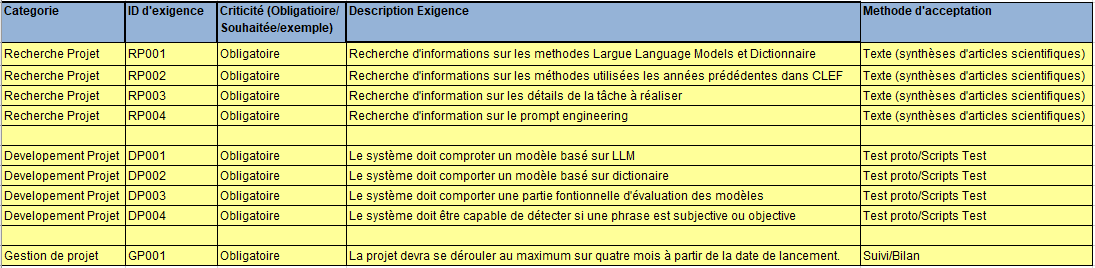
\includegraphics[height=4.2cm]{capture_besoin.png}\\
\tiny
 Source : référentiel projet - Lien : lien github ici ----------------ATTENTION---------------------
\end{center}

\chapter{Organisation}
\section{Organisation globale}

\subsection{Organisation du travail}
\qquad Le projet se découpe en deux phases principales que nous abordons chacune avec leur propre méthode de management de projet.

La première phase est la phase de recherche. Nous réalisons un Etat de l'Art des méthodes utilisées par les équipes de l'année 2023, des recherches effectuées sur la détection automatique de la subjectivité ainsi que l'avancement de la recherche sur les technologies qui pourraient nous être utiles (tels que le prompt engineering). Afin de pouvoir aisément diriger nos recherches, nous adoptons ici une méthode KanBan avec des discussions interne et avec la cliente de manière régulière.

Après avoir effectué le choix de technologie nous basculeront vers une méthode AGILE pour mieux convenir aux besoins de management de la phase de développement. (mettre un pointeur vers quelque chose qui va changer? maybe des milestones de la méthode agile?) <-------------------------

\subsection{Communication avec le client}
\qquad Afin d'assurer une bonne communication avec la cliente, il a été conclu pendant la réunion de lancement du projet que des réunions de 5 à 15 minutes seront faites en fin de journées sur chacun des deux jours prévus pour le projet dans la semaine, lundi et mardi.Ces réunions rapides nous permettent de tenir la cliente informé 
sur l'avancement du projet et de définir dynamiquement les tâches à effectuer par la suite. Hors des réunions, nous communiquons par mails avec tous les participants en copie (cf XXX titre de la partie qualité). <---------

Nous utilisons une communication par mail hors-réunions selon les besoins de gestion qui peuvent subvenir.

\subsection{communication avec l'UE Management} 

\subsection{communication avec les AMO} 

\section{Organisation interne de l'équipe}
\subsection{Communication}
\qquad Afin de faciliter la communication interne, nous utilisons la plateforme de messagerie instantanée: Discord. L'objectif de Discord est de nous permettre de communiquer rapidement et de se partager des documents avant validation. Pour s'assurer que le serveur Discord reste organisé, chaque membre du groupe a les permissions nécessaires afin de créer, remanier ou supprimer les canaux de discussion.
Au besoin, selon les tâches en cours, nous nous rassemblons en présentiel pour collaborer.

\subsection{Suivi des tâches}
\qquad Nous utilisons un outil de gestion de projet en ligne inspiré de la méthode KanBan : Trello. Il va nous permettre d’indiquer les différentes tâches à faire, les tâches en cours ainsi que les tâches finies, afin d’avoir un réel suivi sur le projet pour l’ensemble des membres du groupe. Le Trello nous sert aussi à regrouper tous les points à aborder et les informations importantes transmises lors des réunions avant de les transcrire proprement dans les comptes-rendus de réunions.

Référenctiel de structure projet : Nous établissons un document excel qui permet de sauvegarder la structuration de projet au niveau OBS (organisation breakdown structure), PBS (project breakdown structure), WBS (work breakdown structure), diagramme de gantt intiale et un diagramme de gantt que nous mettons à jour au fur et à mesure des besoins..

\subsection{Gestion des ressources et de la production}
\qquad Pour gérer nos ressources et nos productions, nous utilisons un système de contrôle de version distribué populaire : github. Nous déposons dans ce dépôt tous les documents validés d'après nos règles de qualité (cf chapitre mon cul).<------------------------------------------------------- La gestion automatique des versions fournie par git et github nous permettent de pouvoir constamment accéder aux versions antérieures de chaque document sans avoir à nous préoccuper de le superviser. Le dépôt est visible publiquement afin de permettre aux parties prenantes de pouvoir consulter les ressources qui les intéressent.

Lien github : \url{https://github.com/fghjklm/Projet_M1_CheckThat-}

En parallèle, nous utilisons le logiciel Zotero afin de regrouper tous les articles potentiellement liés à nos objectifs. Nous effectuons des synthèses des plus pertinents qui se retrouvent dans le github.
Lien github des synthèses. <------------------------------------

\chapter{Phase de Recherche}
\section{Modèles et résultats des équipes de CLEF 2023}
CLEF : Conference and Labs of the Evaluation Forum.\\
\vspace{0mm}
\qquad L'accès aux rapports des équipes de CLEF 2023 est une opportunité de taille dans la réalisation de notre projet. Nous explorons les méthodes qui ont été utilisées et essayons d'extraire les informations utiles : les modèles, méthodes de fine-tuning ou les raisons des mauvais résultats de certaines équipes.

\section{État de l'art de la détection automatique de la subjectivité}
\qquad Nous effectuons également un état de l'art de la détection automatique de la subjectivité afin découvrir s'il existe des pistes différentes de celles explorées par les équipes de l'an dernier.
lien vers github synthèse des articles <----------------


\section{Avancement de la recherche sur le prompt engeeniring}
\qquad Il est quasiment certain que nous auront à utiliser le prompt engeeniring lors du dev, c'est pourquoi nous effectuons des recherches afin de trouver les méthodes les plus efficaces de prompt engeeniring. L'objectif est de perfectionner les requêtes que nous formulerons au LLM sélectionné dans le choix de technologie.
 (lien vers github rapport choix de techno) <----------------



\chapter{Phase de développement}
\centerline{En construction - Sera établi dans une version future du Plan Projet.}

\chapter{Contrôle Qualité}
\centerline{En construction}


\chapter{ État actuel du projet}
\qquad Dans cette section, nous présentons des liens vers les ressources actuelles du projet, structurées sur un dépôt github (cliquez sur les bouttons représentés par <- Boutton ->), vous y trouverez le référentiel de structure du projet, le diagramme de Gantt, les différentes versions de ce document et les avancements de la recherche et du développement.

\section{Référentiel de structure du projet}
\qquad Le référentiel du plan projet, comprenant l'organisation de la structure à travers l'Organisation Breakdown Structure (OBS), le Project Breakdown Structure (PBS), le Work Breakdown Structure (WBS), est accessible ici :
\href{https://github.com/fghjklm/Projet_M1_CheckThat-/tree/main/referentiel_projet}{<- Référentiel projet ->}

\section{Versions du Plan Projet}
\qquad Les autres versions du Plan Projet sont accessibles ici :
\href{https://github.com/fghjklm/Projet_M1_CheckThat-/tree/main/plan_projet}{<- Plan Projet ->}

\section{Diagramme de Gantt actuel}
\qquad Vous pouvez consulter le diagramme de Gantt actuel pour suivre l'évolution du projet en utilisant ce lien :
\href{https://github.com/fghjklm/Projet_M1_CheckThat-/tree/main/gantt}{<- Gantt ->}

\section{Avancement de la recherche}
\qquad Pour voir les progrès de notre recherche, veuillez consulter ce dossier :
\href{https://github.com/fghjklm/Projet_M1_CheckThat-/tree/main/articles}{<- La Recherche ->}

\section{Avancement du développement}
\qquad L'avancement du développement du projet est disponible dans le dossier suivant :
\href{https://github.com/fghjklm/Projet_M1_CheckThat-/tree/main/code}{<- Le développement ->}

\section{Autres ressources}
\qquad Toutes les autres ressources liées au projet, telles que les rapports intermédiaires, les documents de conception, et les résultats des tests, sont également disponibles dans notre page GitHub.


\chapter{\quad Bilan}
\centerline{En construction - Sera établi dans la version 3 du Plan Projet.}
\end{document}
